% Fig. 2, Introduction overview. v1 draft image; replaced by paper/figures/cvpr_v1/fig02_overview.pdf when ready.
\begin{figure*}[t]
\centering
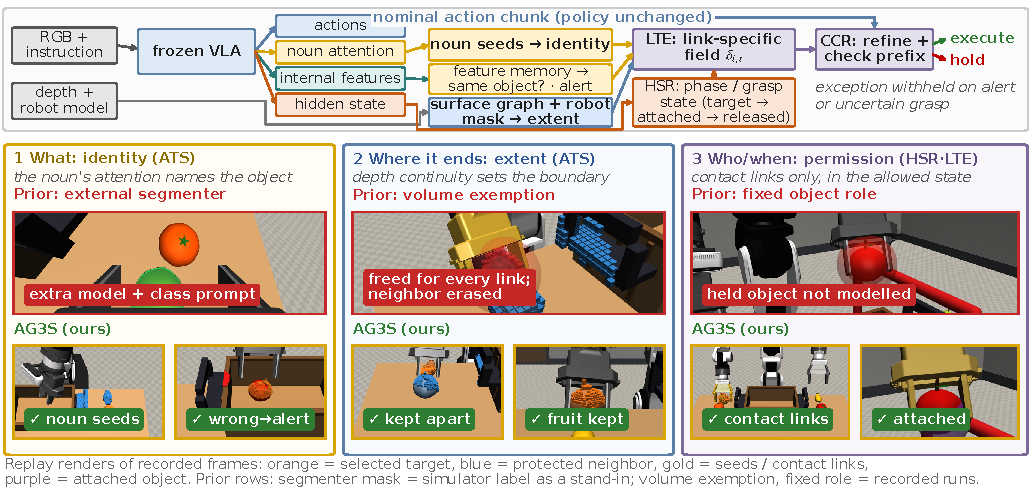
\includegraphics[width=\textwidth]{../figures/cvpr_v1/fig02_overview.pdf}
\caption{\textbf{One frozen VLA decides what may be touched, where that surface ends, and by which link, when.}
\emph{Top:} \sys\ reads noun attention, internal features, and hidden state from the same frozen policy that produces the action chunk, and turns them with depth into one link-specific contact representation that constrained refinement (CCR) enforces.
\emph{Bottom, each against the closest prior practice.} \emph{Identity:} eligible noun-attention patches seed the object, and centered features tell whether it is still the same one. \emph{Extent:} depth continuity and a rendered robot mask bound the surface, so the touching fruit stays protected and the fruit between the fingers is kept, where radius growth and a volume mask swallow one and erase the other. \emph{Permission:} only the contact links of the active hand may enter it; after a confirmed grasp the object becomes carried geometry and, on release, an obstacle again. The permission panels are recorded frames of the coarse-extent configuration, which shares this contact interface.}
\label{fig:overview}
\end{figure*}
